\documentclass[a4paper,11pt]{article}

\usepackage{amsmath,amssymb}
\usepackage{graphicx}
\usepackage{geometry}
\usepackage{siunitx}
\usepackage{hyperref}
\geometry{margin=2.5cm}
\sisetup{round-mode=figures,round-precision=3}

\title{MATH36031 Project 2:\\Fox--Rabbit Chase on a Circular Fence}
\author{Shivsaransh Thakur}
\date{\today}

\begin{document}
\maketitle

\section{Introduction}

We consider a pursuit problem on a circular fence of radius \SI{800}{\metre}. A fox starts at the origin $F_0=(0,0)$ and a rabbit starts at $R_0=(0,800)$ on the fence. The rabbit runs along the fence towards a fixed burrow located at
\[
B = 800\bigl(\sin(\pi/3),\cos(\pi/3)\bigr),
\]
while the fox aims to catch the rabbit by exploiting a gap in the fence at $G=(0,300)$ and a straight fence segment between $A=(380,600)$ and $E=(450,320)$. The fox catches the rabbit if the distance between them becomes less than \SI{0.1}{\metre}.

The project has two parts:
\begin{itemize}
  \item \textbf{Question 1 (constant speeds):} the fox and rabbit move with constant speeds $s_f=\SI{16}{m/s}$ and $s_r=\SI{13}{m/s}$.
  \item \textbf{Question 2 (diminishing speeds):}
  \begin{align*}
    s_f(d_f) &= s_{f0} e^{-\mu_f d_f}, &
    s_r(d_r) &= s_{r0} e^{-\mu_r d_r},
  \end{align*}
  with $s_{f0}=\SI{16}{m/s}$, $s_{r0}=\SI{13}{m/s}$, $\mu_f=2\times 10^{-4}$ and $\mu_r=8\times 10^{-4}$, where $d_f$ and $d_r$ are the distances travelled by fox and rabbit respectively.
\end{itemize}
The aim is to determine whether the fox captures the rabbit before it reaches the burrow, and to quantify the time and distance travelled by the fox in both regimes.

\section{Mathematical formulation}

\subsection{Geometry}

The circular fence has radius $R=\SI{800}{\metre}$. We use a global Cartesian frame with the origin at $F_0=(0,0)$ and the initial rabbit position
\[
R_0 = (0,R) = (0,800).
\]
We parameterise the fence by angle $\theta$ with
\[
(x(\theta),y(\theta)) = \bigl(R\sin\theta, R\cos\theta\bigr), \qquad \theta\in[0,2\pi).
\]
The rabbit starts at $\theta=0$ and runs towards the burrow at angle $\theta_B=\pi/3$. The total arc length to the burrow is
\[
S_B = R\theta_B = 800\frac{\pi}{3} \approx \SI{837.758}{\metre}.
\]

The fox always moves in the plane. Its motion is piecewise defined by target points:
\begin{itemize}
  \item \textbf{Phase 1:} run directly from $F_0$ to the gap $G$.
  \item \textbf{Phase 2:} from then on, if the line segment from the fox to the rabbit intersects the fence segment $AE$, the fox runs towards $A$; otherwise it runs directly towards the rabbit.
\end{itemize}

\subsection{Rabbit motion}

In the constant-speed case the rabbit moves at speed $s_r=\SI{13}{m/s}$, so its arc length at time $t$ is $s(t)=s_r t$ and the angular position is
\[
\theta(t) = \min\left(\frac{s_r t}{R},\theta_B\right).
\]
The corresponding Cartesian position is
\[
R(t) = \bigl(x_r(t),y_r(t)\bigr)
       = \bigl(R\sin\theta(t), R\cos\theta(t)\bigr).
\]
The time to reach the burrow is
\[
T_B^{\text{const}} = \frac{S_B}{s_r}
= \frac{800(\pi/3)}{13} \approx \SI{64.44}{\second}.
\]

In the diminishing-speed case we model the rabbit by its cumulative distance $d_r(t)$ along the fence, evolving as
\[
\frac{d d_r}{dt} = s_r(d_r) = s_{r0} e^{-\mu_r d_r}.
\]
The position is then obtained from the distance $d_r$ via
\[
\theta(t) = \min\left(\frac{d_r(t)}{R},\theta_B\right), \qquad
R(t)= \bigl(R\sin\theta(t),R\cos\theta(t)\bigr).
\]

\subsection{Fox motion}

Let $F(t)=(x_f(t),y_f(t))$ denote the fox position. At any time we choose a target point $T(t)$ according to the phase logic described above. The (unit) direction of motion is
\[
\hat{u}(t) = \frac{T(t)-F(t)}{\|T(t)-F(t)\|},
\]
whenever $F(t)\neq T(t)$; otherwise the velocity is set to zero.

\paragraph{Question 1 (constant speed).} The fox moves with constant speed $s_f=\SI{16}{m/s}$:
\[
\frac{dF}{dt} = s_f\,\hat{u}(t).
\]

\paragraph{Question 2 (diminishing speed).} We introduce the cumulative fox distance $d_f(t)$ and set
\[
\frac{d d_f}{dt} = s_f(d_f) = s_{f0} e^{-\mu_f d_f},\qquad
\frac{dF}{dt} = s_f(d_f)\,\hat{u}(t).
\]

\subsection{Capture and stopping conditions}

The simulation is stopped when one of the following events occurs:
\begin{itemize}
  \item \textbf{Capture:} $\|F(t)-R(t)\| \leq \SI{0.1}{\metre}$.
  \item \textbf{Rabbit reaches burrow:} in the constant-speed case, $t \geq T_B^{\text{const}}$; in the diminishing-speed case, $d_r(t)\geq S_B$.
\end{itemize}
We record the stopping time $T$, the fox position $F(T)$ and the distances $d_f(T)$ (and $d_r(T)$ in Question 2).

\section{Numerical method}

All simulations were implemented in \textsc{MATLAB} using the built-in solver \texttt{ode45}, which is an explicit Runge--Kutta (4,5) method with adaptive time stepping. The implementation is structured into small, unit-tested components:

\begin{itemize}
  \item Geometric primitives: segment intersection and line-of-sight blocking for the fence segment $AE$.
  \item Target selection logic for the fox.
  \item Separate modules for constant-speed and distance-dependent-speed models.
  \item ODE right-hand sides and event functions for both questions.
  \item High-level drivers \texttt{simulate\_constant\_case} and \texttt{simulate\_variable\_case} that orchestrate the phases (running to $G$, then chasing).
\end{itemize}

For both questions, the ODE solver is used with relative tolerance \texttt{RelTol = 1e-8} and absolute tolerance \texttt{AbsTol = 1e-10}. Events are implemented via custom event functions passed to \texttt{odeset}. The code is organised under \texttt{src/} with unit tests under \texttt{tests/}, executed via \texttt{matlab.unittest}.

\section{Results}

\subsection{Constant-speed case (Question 1)}

In the constant-speed regime, the rabbit reaches the burrow in
\[
T_B^{\text{const}} \approx \SI{64.44}{\second}.
\]
The numerical simulation confirms this value to within the solver tolerance. The fox distance travelled by this time is
\[
d_f(T_B^{\text{const}}) \approx \SI{1031.1}{\metre},
\]
and its position is approximately
\[
F(T_B^{\text{const}}) \approx (\SI{585.51}{\metre},\,\SI{492.84}{\metre}).
\]
The separation between fox and rabbit at this time remains well above the capture threshold of \SI{0.1}{\metre}. Thus, in the constant-speed case
\[
\text{the fox does not capture the rabbit before it reaches the burrow.}
\]

Figure~\ref{fig:constant_paths} shows the trajectories of the fox and rabbit, together with the circular fence, the gap $G$, the fence segment $AE$ and the burrow.

\begin{figure}[h]
\centering
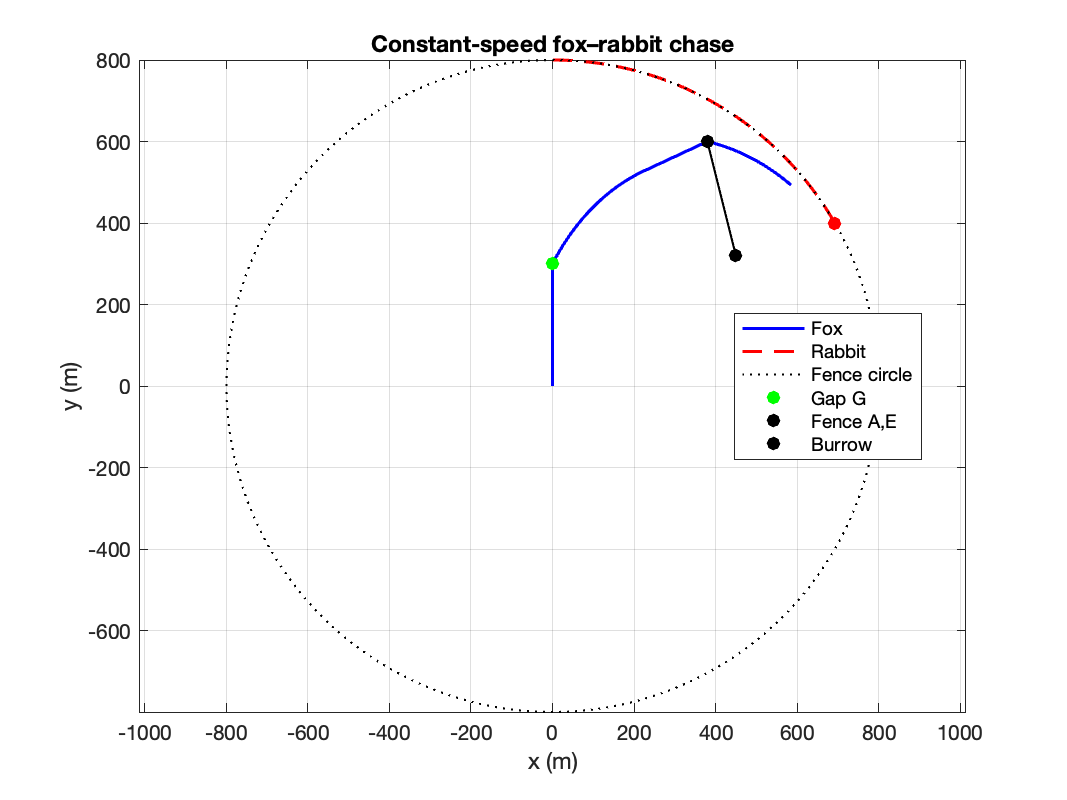
\includegraphics[width=0.7\textwidth]{constant_case_paths.png}
\caption{Fox and rabbit paths in the constant-speed case. The fox runs to the gap $G$ and then attempts to chase, but the rabbit reaches the burrow first.}
\label{fig:constant_paths}
\end{figure}

\subsection{Diminishing-speed case (Question 2)}

In the diminishing-speed regime, the cumulative rabbit distance reaches the required arc length $S_B\approx\SI{837.76}{\metre}$ at time
\[
T^{\text{var}} \approx \SI{91.79}{\second},
\]
which is significantly larger than $T_B^{\text{const}}$ due to the exponential decay of the rabbit's speed. The simulation yields
\begin{align*}
  d_f(T^{\text{var}}) &\approx \SI{1287.7}{\metre}, \\
  d_r(T^{\text{var}}) &\approx \SI{837.76}{\metre}, \\
  F(T^{\text{var}})   &\approx (\SI{0}{\metre},\,\SI{300}{\metre}) = G.
\end{align*}
Thus the fox ends up at the gap $G$ precisely when the rabbit reaches the burrow, but again the separation is larger than \SI{0.1}{\metre}, so no capture occurs:
\[
\text{the fox does not capture the rabbit in the diminishing-speed case either.}
\]

Figure~\ref{fig:variable_paths} shows the trajectories in the variable-speed case. Compared to Figure~\ref{fig:constant_paths}, both fox and rabbit spend longer near their respective targets due to the decaying speeds, but the qualitative geometry remains similar.

\begin{figure}[h]
\centering
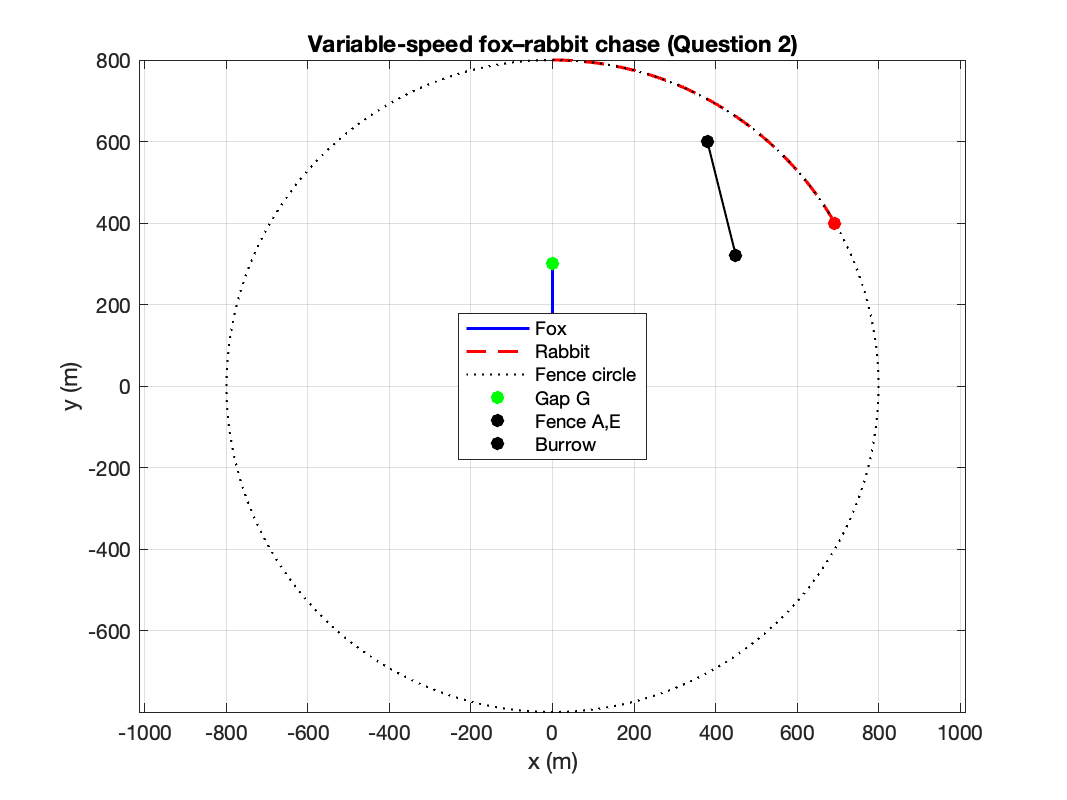
\includegraphics[width=0.7\textwidth]{variable_case_paths.png}
\caption{Fox and rabbit paths in the variable-speed case. Both speeds decay exponentially with distance, so the rabbit takes longer to reach the burrow, but the fox also slows, and again fails to capture.}
\label{fig:variable_paths}
\end{figure}

\section{Discussion}

The results show that, in this geometric configuration, the presence of the gap $G$ and fence segment $AE$ is not sufficient for the fox to intercept the rabbit, even when it starts faster both in the constant-speed and diminishing-speed regimes. In the constant-speed case, the key limiting factor is the geometry: the rabbit effectively ``cuts the corner'' along the circle, while the fox must first reach the gap and then manoeuvre around the fence.

In the diminishing-speed case, both animals slow down with distance, but the relative advantage of the fox is not large enough to compensate for the geometric disadvantage. The fox arrives at the gap $G$ at approximately the same time that the rabbit is close to the burrow and cannot close the remaining distance before the rabbit reaches safety.

\section{Conclusions}

We formulated the fox--rabbit chase as a piecewise-smooth dynamical system with event-based stopping criteria and implemented it in \textsc{MATLAB} using modular, unit-tested components. For both the constant-speed and diminishing-speed models, the numerical simulations indicate that the fox fails to capture the rabbit before it reaches the burrow. The framework developed here can be extended to explore alternative parameter regimes, different fence geometries or stochastic perturbations to the motion.

\end{document}
